\documentclass[a4paper,12pt,final,oneside,openright]{article}
\usepackage{report}

\newcommand{\reporttitle}{Computer graphics and interaction}
\newcommand{\enseignants}{
Christopher Peters
}

\newcommand{\reportauthor}{
Rémi Domingues}
% \newcommand{\hexanome}{H4211}
\newcommand{\reportsubject}{}
\newcommand{\stagetopic}{Raytracing}
\newcommand{\dateperiod}{April $6^{th}$ - May $19^{th}$}
\newcommand{\HRule}{\rule{\linewidth}{0.5mm}}
\setlength{\parskip}{1ex} % Espace entre les paragraphes

\hypersetup{
    pdftitle={\reporttitle},%
    pdfauthor={\reportauthor},%
    pdfsubject={\reportsubject},%
    pdfkeywords={}
}

\title{\reporttitle}
\author{\reportauthor}

\setlongtables
\usepackage[font=small,skip=0pt]{caption}
\usepackage{algorithm}
\usepackage{algpseudocode}


%\setcounter{tocdepth}{4}
\begin{document}
    \renewcommand{\chaptername}{} %\renewcommand{\thechapter}{}
    \renewcommand{\contentsname}{Contents}

    \pagestyle{empty}
    \pagenumbering{arabic}
    % Inspiré de http://en.wikibooks.org/wiki/LaTeX/Title_Creation
\begin{center}
	\begin{minipage}[t]{0.48\textwidth}
	  \begin{flushleft}
	    
\includegraphics [width=30mm]{img/logo_kth.jpg} \\[0.1cm]
		Kungliga Tekniska Högskolan\\
		Valhallavägen 79\\
		100 44 Stockholm
	  \end{flushleft}
	\end{minipage}
	\begin{minipage}[t]{0.48\textwidth}
	  \begin{flushright}
	  \end{flushright}
	\end{minipage} \\[1cm]

	\textsc{\Large \reportsubject}\\[0.3cm]
	\HRule \\[0.4cm]
	{\Huge \bfseries \reporttitle}\\[0.3cm]
	{\LARGE \bfseries «~\stagetopic~»}\\[0.3cm]
	{\Large \dateperiod}\\[0.4cm]
	\HRule \\[1.5cm]

	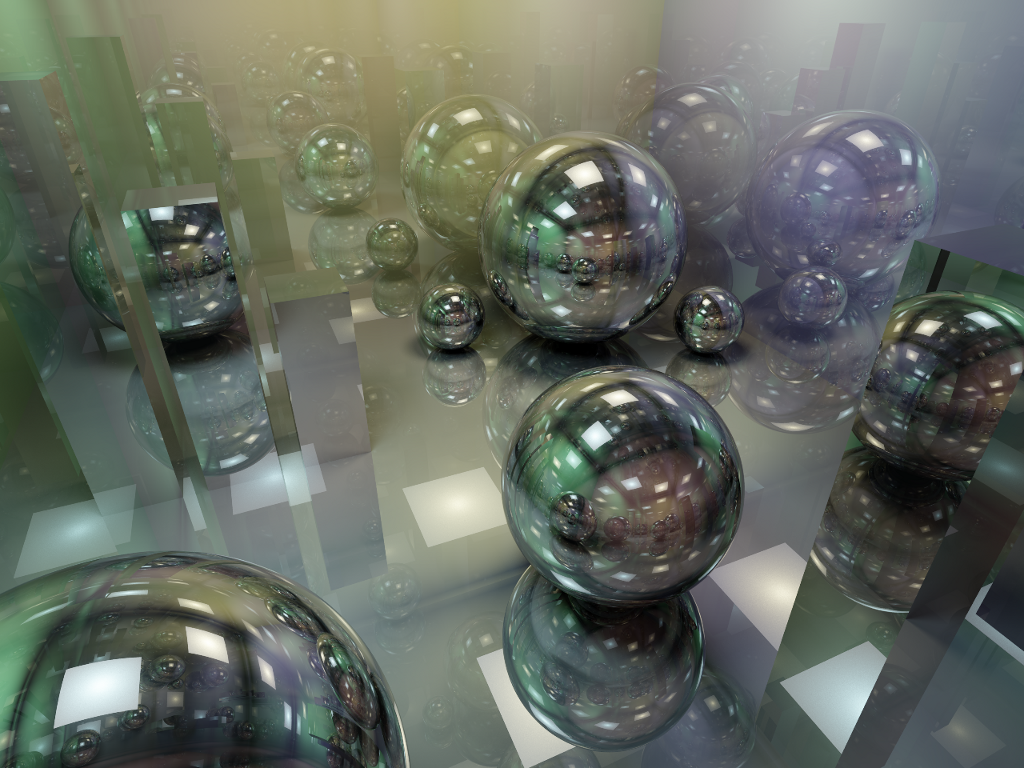
\includegraphics [width=0.65\linewidth]{img/icon.png} \\[1.5cm]
	\begin{minipage}[t]{0.5\textwidth}
	  \begin{flushleft} \large
	    \emph{Author}\\
	    \reportauthor
	  \end{flushleft}
	\end{minipage}
	\begin{minipage}[t]{0.4\textwidth}
	  \begin{flushright} \large
	    \emph{Teachers} \\
	    \enseignants
	  \end{flushright}
	\end{minipage}

	\vfill
	\footnotesize{Scholar year 2014-2015}
\end{center}

    \pagebreak
    \sloppy          % Justification moins stricte : des mots ne dépasseront pas des paragraphes

    %\frontmatter
    \thispagestyle{empty}
    %\tableofcontents
    \addtocontents{toc}{\protect\thispagestyle{empty}}
    \pagebreak

    %\mainmatter
    \pagestyle{headings}
    %\renewcommand{\chaptermark}[1]{\markboth{\MakeUppercase{\chaptername\ \thechapter.\ #1}}{}}
    %\renewcommand{\sectionmark}[1]{\markright{\thesection{} #1}}

    \section*{Introduction}
This document describes the implementation and output of a raytracer supporting triangles and spheres, direct light and soft shadows, diffuse, specular, semi-specular and glass materials, anti-aliasing and multithreading.

The model used in this experiment is the Cornell Box available at \url{http://www.graphics.cornell.edu/online/box}.

\setcounter{section}{0}

\section{Ray-triangle intersection}
By representing rays as lines in 3D, defined by a starting point and a direction (3D vector), we are able to compute the intersection between a ray and a triangle as described below.
This can be expressed as a line-plane intersection, where we check that the intersection lies in the triangle using the vectors $\vec{T_1T_3}$ and $\vec{T_1T_2}$.

\begin{figure}[H]
\centering
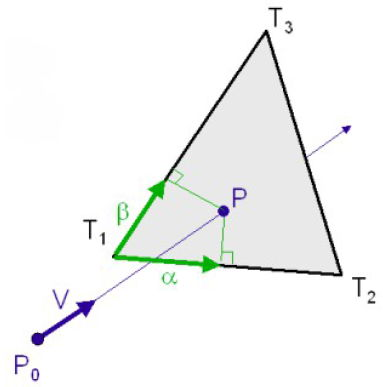
\includegraphics[width=0.2\linewidth]{img/ray.jpg}
\caption{Ray-triangle intersection}
\end{figure}

These computations are implemented in the following method, which returns the intersection (t u v) between a ray described by a starting point and a direction and a triangle, with t distance and u and v triangle delimiters.
\begin{lstlisting}
vec3 GetIntersection(vec3 start, vec3 dir, Triangle triangle) {
	vec3 v0 = triangle.v0;
	vec3 v1 = triangle.v1;
	vec3 v2 = triangle.v2;
	vec3 e1 = v1 - v0;
	vec3 e2 = v2 - v0;
	vec3 b = start - v0;
	mat3 A(-dir, e1, e2);
	return glm::inverse(A) * b;
}
\end{lstlisting}


\section{Tracing Rays}
Using the pinhole camera model, rays are traced from the camera, lying in position (0, 0, -3) and directed toward the \textit{z} axis. Their closest intersection are then computed in order to display the closest triangle.

A focal length equal to the screen width has been used. With $width = height = 500$, we obtain the following field of views:
\begin{equation}
\begin{split}
FOV_{vertical} = 2 * arctan(\frac{\frac{height}{2}}{f}) = 2 * arctan(\frac{500}{500}) = 90^\circ\\
FOV_{horizontal} = 2 * arctan(\frac{\frac{width}{2}}{f}) = 2 * arctan(\frac{500}{500}) = 90^\circ
\end{split}
\end{equation}

\begin{figure}[H]
\centering
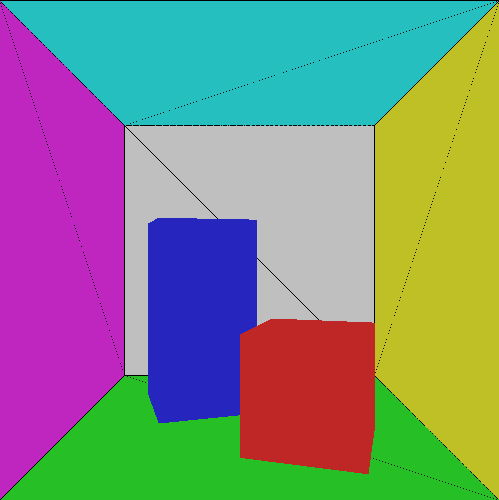
\includegraphics[width=0.3\linewidth]{img/init.jpg}
\caption{Rendering output}
\end{figure}

\section{Moving the Camera}
A camera rotation on the \textit{y}-axis has been introduced by multiplying the rays direction vector by the rotation matrix below, with $\theta$ the camera angle.
\begin{equation}
R = \left( \begin{array}{ccc}
\cos(\theta) & 0 & \sin(\theta) \\
0 & 1 & 0 \\
-\sin(\theta) & 0 & \cos(\theta) \end{array} \right)
\end{equation}

Then, obtaining the axes direction using equation \ref{eq:axes}, we can apply a camera translation by adding the corresponding axes direction to the camera position.
\begin{equation}
\label{eq:axes}
\begin{split}
\vec{x} = ( R[0][0], R[0][1], - R[0][2] )\\
\vec{y} = ( R[1][0], R[1][1], R[1][2] )\\
\vec{z} = ( - R[2][0], R[2][1], R[2][2] )
\end{split}
\end{equation}

These translations and rotations are triggered by pressing the arrow keys.

\begin{figure}[H]
\minipage{0.24\textwidth}
    \centering
    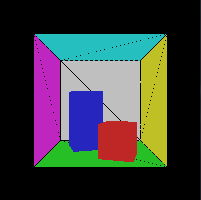
\includegraphics[width=\linewidth]{img/backward.jpg}
    \caption{Backward translation}
\endminipage\hfill
\minipage{0.24\textwidth}
    \centering
    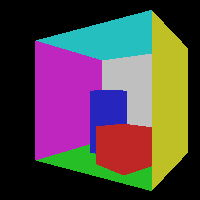
\includegraphics[width=\linewidth]{img/right.jpg}
    \caption{Right rotation and translation}
\endminipage\hfill
\minipage{0.24\textwidth}
    \centering
    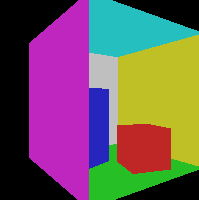
\includegraphics[width=\linewidth]{img/left.jpg}
    \caption{Left rotations and translations}
\endminipage\hfill
\minipage{0.24\textwidth}
    \centering
    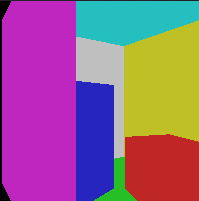
\includegraphics[width=\linewidth]{img/forward.jpg}
    \caption{Forward translation}
\endminipage\hfill
\end{figure}

\section{Illumination}
\subsection{Direct light}
Direct light is computed by estimating the light power reaching a triangle. This data is processed for every intersection computed in sections 2 and 3. This estimation only does not take into account obstacles between the light source and the intersection, which is why the renderings below do not contain any shadow.

The power \textit{D} is explained in equation \ref{eq:power}, using \textit{P} the power of the light source, i.e. energy per time unit for each color component (14.f * vec3( 1, 1, 1 ) for example), r the distance from the intersection to the light source, $\hat{n}$ the normal of the triangle and $\hat{r}$ a unit vector describing the direction from the surface point to the light source.
\begin{equation}
\label{eq:power}
D = \frac{P * max(\hat{r} . \hat{n}, 0)}{4 \pi r^2}
\end{equation}

Using the same translation as described in section 4, the light source can be moved in the 6 possible directions using W, A, S, D, Q and E.

\begin{figure}[H]
\minipage{0.33\textwidth}
    \centering
    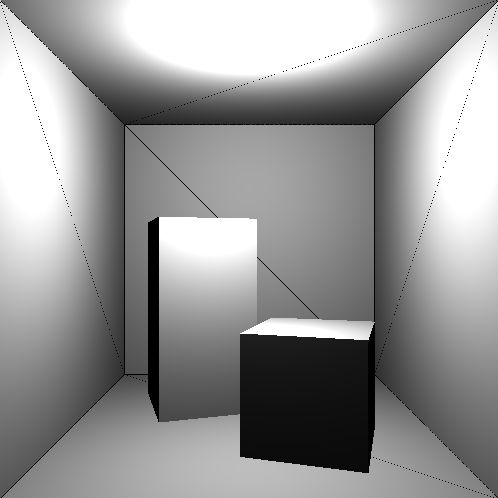
\includegraphics[width=\linewidth]{img/light1.jpg}
    \caption{Direct light}
\endminipage\hfill
\minipage{0.33\textwidth}
    \centering
    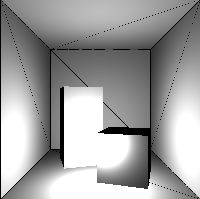
\includegraphics[width=\linewidth]{img/light2.jpg}
    \caption{Moving down}
\endminipage\hfill
\minipage{0.33\textwidth}
    \centering
    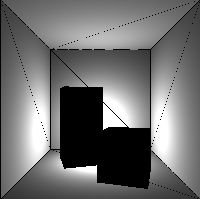
\includegraphics[width=\linewidth]{img/light3.jpg}
    \caption{Moving forward}
\endminipage\hfill
\end{figure}

Multiplying the triangle color by the power \textit{D} for each color component reaching the intersection, we obtain the following renderings.

\begin{figure}[H]
\minipage{0.33\textwidth}
    \centering
    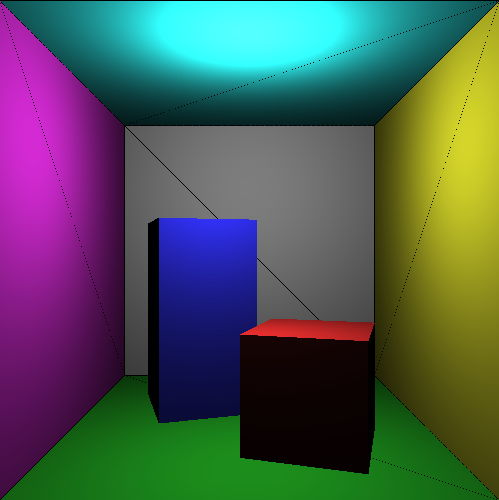
\includegraphics[width=\linewidth]{img/light_col1.jpg}
    \caption{Direct light}
\endminipage\hfill
\minipage{0.33\textwidth}
    \centering
    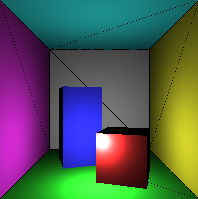
\includegraphics[width=\linewidth]{img/light_col2.jpg}
    \caption{Moving down}
\endminipage\hfill
\minipage{0.33\textwidth}
    \centering
    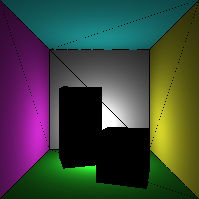
\includegraphics[width=\linewidth]{img/light_col3.jpg}
    \caption{Moving forward}
\endminipage\hfill
\end{figure}


\subsection{Direct shadows}
In order to make this scene more realistic, we render shadows by tracing rays from the light source to our intersections. If the intersection returned is closer than the distance between the intersection and the light source, this mean that light is hidden by another object. Light power is thus set to 0 for each color component.

\begin{figure}[H]
\centering
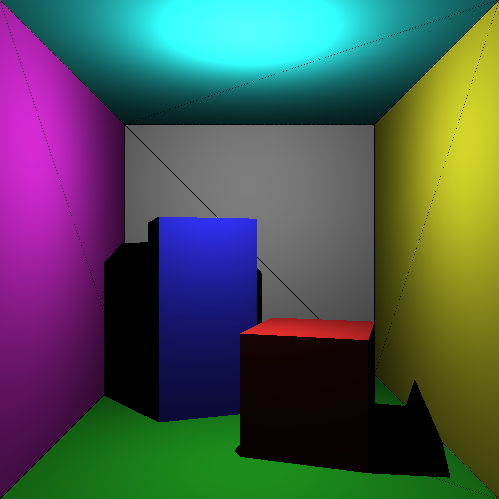
\includegraphics[width=0.35\linewidth]{img/shadows.jpg}
\caption{Direct shadows}
\end{figure}

\subsection{Indirect illumination}
Eventually, to avoid black shadows and simulate the indirect illumination obtained by multiples bounces of rays from the light source, we add an indirect illumination constant to the power received by every intersection.

Note that computing those bounces would result in a rendering much more realistic but also in a loss of performances.

Therefore, the color of a triangle is now computed as follows, with \textit{N} the indirect illumination constant and $\rho$ the RGB vector of a triangle (reflectance).
\begin{equation}
R = \rho * (D+N)
\end{equation}

\begin{figure}[H]
\centering
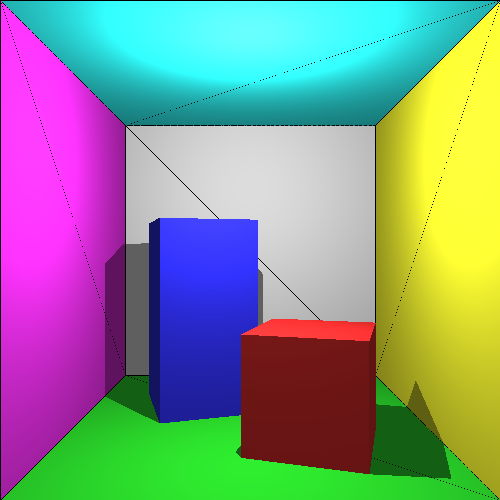
\includegraphics[width=0.35\linewidth]{img/ind_light.jpg}
\caption{Indirect illumination}
\end{figure}
    \section{Spheres}
\begin{figure}[H]
\centering
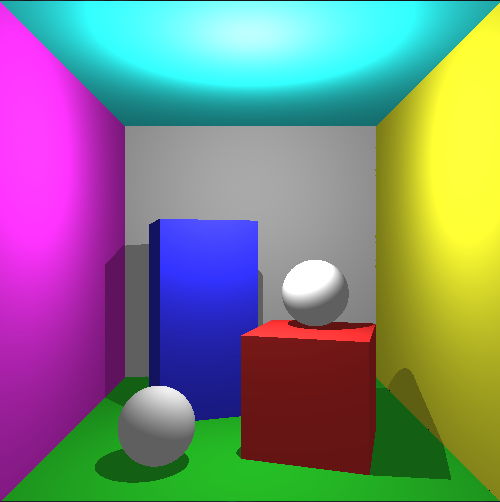
\includegraphics[width=0.4\linewidth]{img/spheres.jpg}
\caption{Spheres (930 ms)}
\end{figure}


\section{Ray-triangle intersection: optimization}
New ray/triangle intersection algorithm:
http://en.wikipedia.org/wiki/M%C3%B6ller%E2%80%93Trumbore_intersection_algorithm (3 times faster, 360ms)


\section{Specular materials}
\begin{figure}[H]
\centering
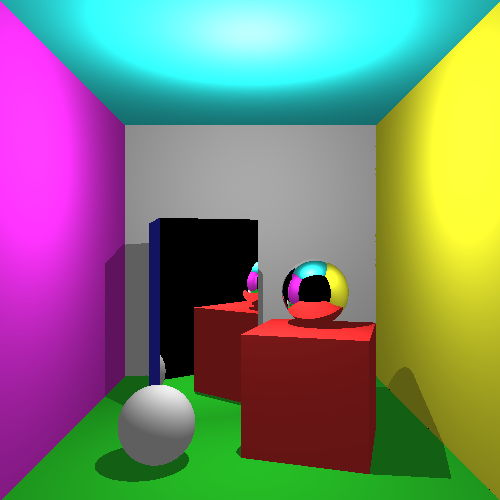
\includegraphics[width=0.4\linewidth]{img/specular.jpg}
\caption{Specular materials}
\end{figure}


\section{Glass - Refraction}
\begin{figure}[H]
\centering
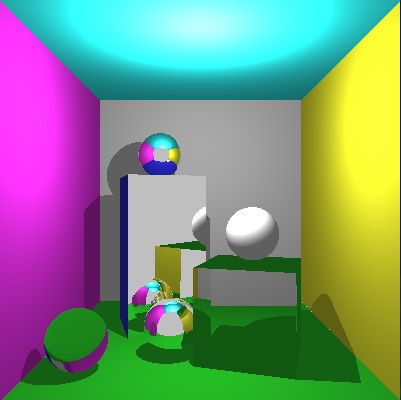
\includegraphics[width=0.4\linewidth]{img/glass_refraction.jpg}
\caption{Refraction through glass (430 ms)}
\end{figure}


\section{Anti-aliasing}
\subsection{Edges detection}


\begin{figure}[H]
\centering
\minipage[t]{0.4\textwidth}
    \centering
    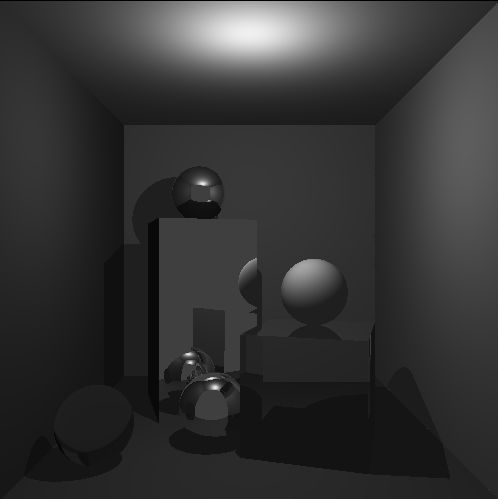
\includegraphics[width=\linewidth]{img/antialiasing/grayscale.jpg}
    \caption{Grayscale scene}
\endminipage
\minipage[t]{0.4\textwidth}
    \centering
    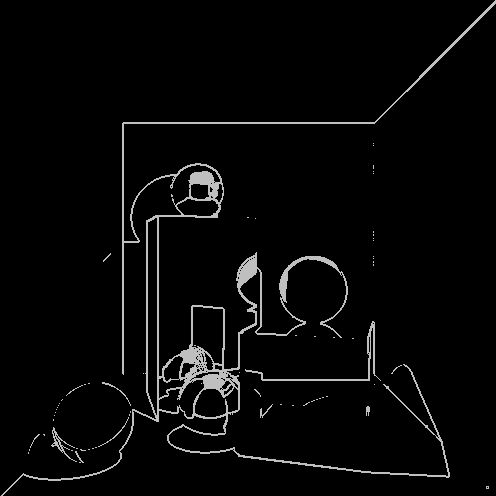
\includegraphics[width=\linewidth]{img/antialiasing/sobel.jpg}
    \caption{Edges detection (Sobel operator)}
\endminipage
\end{figure}


\subsection{Uniform}

\subsection{Stochastic sampling}

They are zoomed
\begin{figure}[H]
\minipage{0.25\textwidth}
    \centering
    
\includegraphics[width=\linewidth]{img/antialiasing/no_aa.png}
    \caption{AA disabled (430 ms)}
\endminipage\hfill
\minipage{0.25\textwidth}
    \centering
    
\includegraphics[width=\linewidth]{img/antialiasing/super8x.png}
    \caption{Uniform 8x (1200 ms)}
\endminipage\hfill
\minipage{0.25\textwidth}
    \centering
    
\includegraphics[width=\linewidth]{img/antialiasing/sto8x.png}
    \caption{Jittered 8x (1250 ms)}
\endminipage\hfill
\minipage{0.25\textwidth}
    \centering
    
\includegraphics[width=\linewidth]{img/antialiasing/sto16x.png}
    \caption{Jittered 16x (1450 ms)}
\endminipage\hfill
\end{figure}


\begin{figure}[H]
\centering
\minipage[t]{0.4\textwidth}
    \centering
    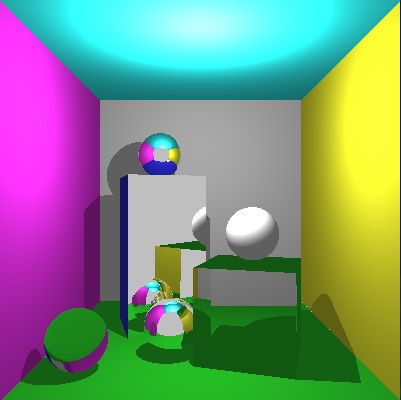
\includegraphics[width=\linewidth]{img/glass_refraction.jpg}
    \caption{Anti-aliasing disabled (430 ms)}
\endminipage
\minipage[t]{0.4\textwidth}
    \centering
    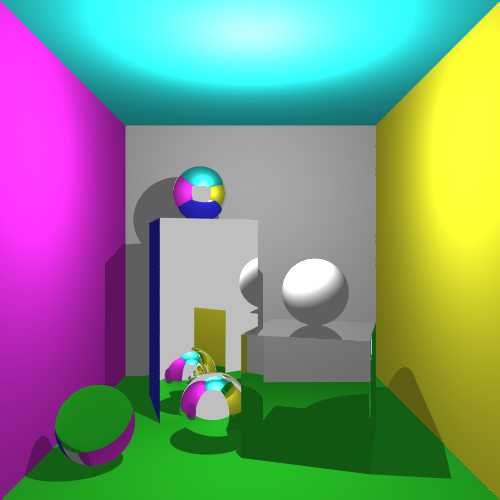
\includegraphics[width=\linewidth]{img/antialiasing/stoAA16x_full.png}
    \caption{Stochastic sampling 16x (1450 ms)}
\endminipage
\end{figure}


\section{Glass - Reflection}
20 bounces
\begin{figure}[H]
\centering
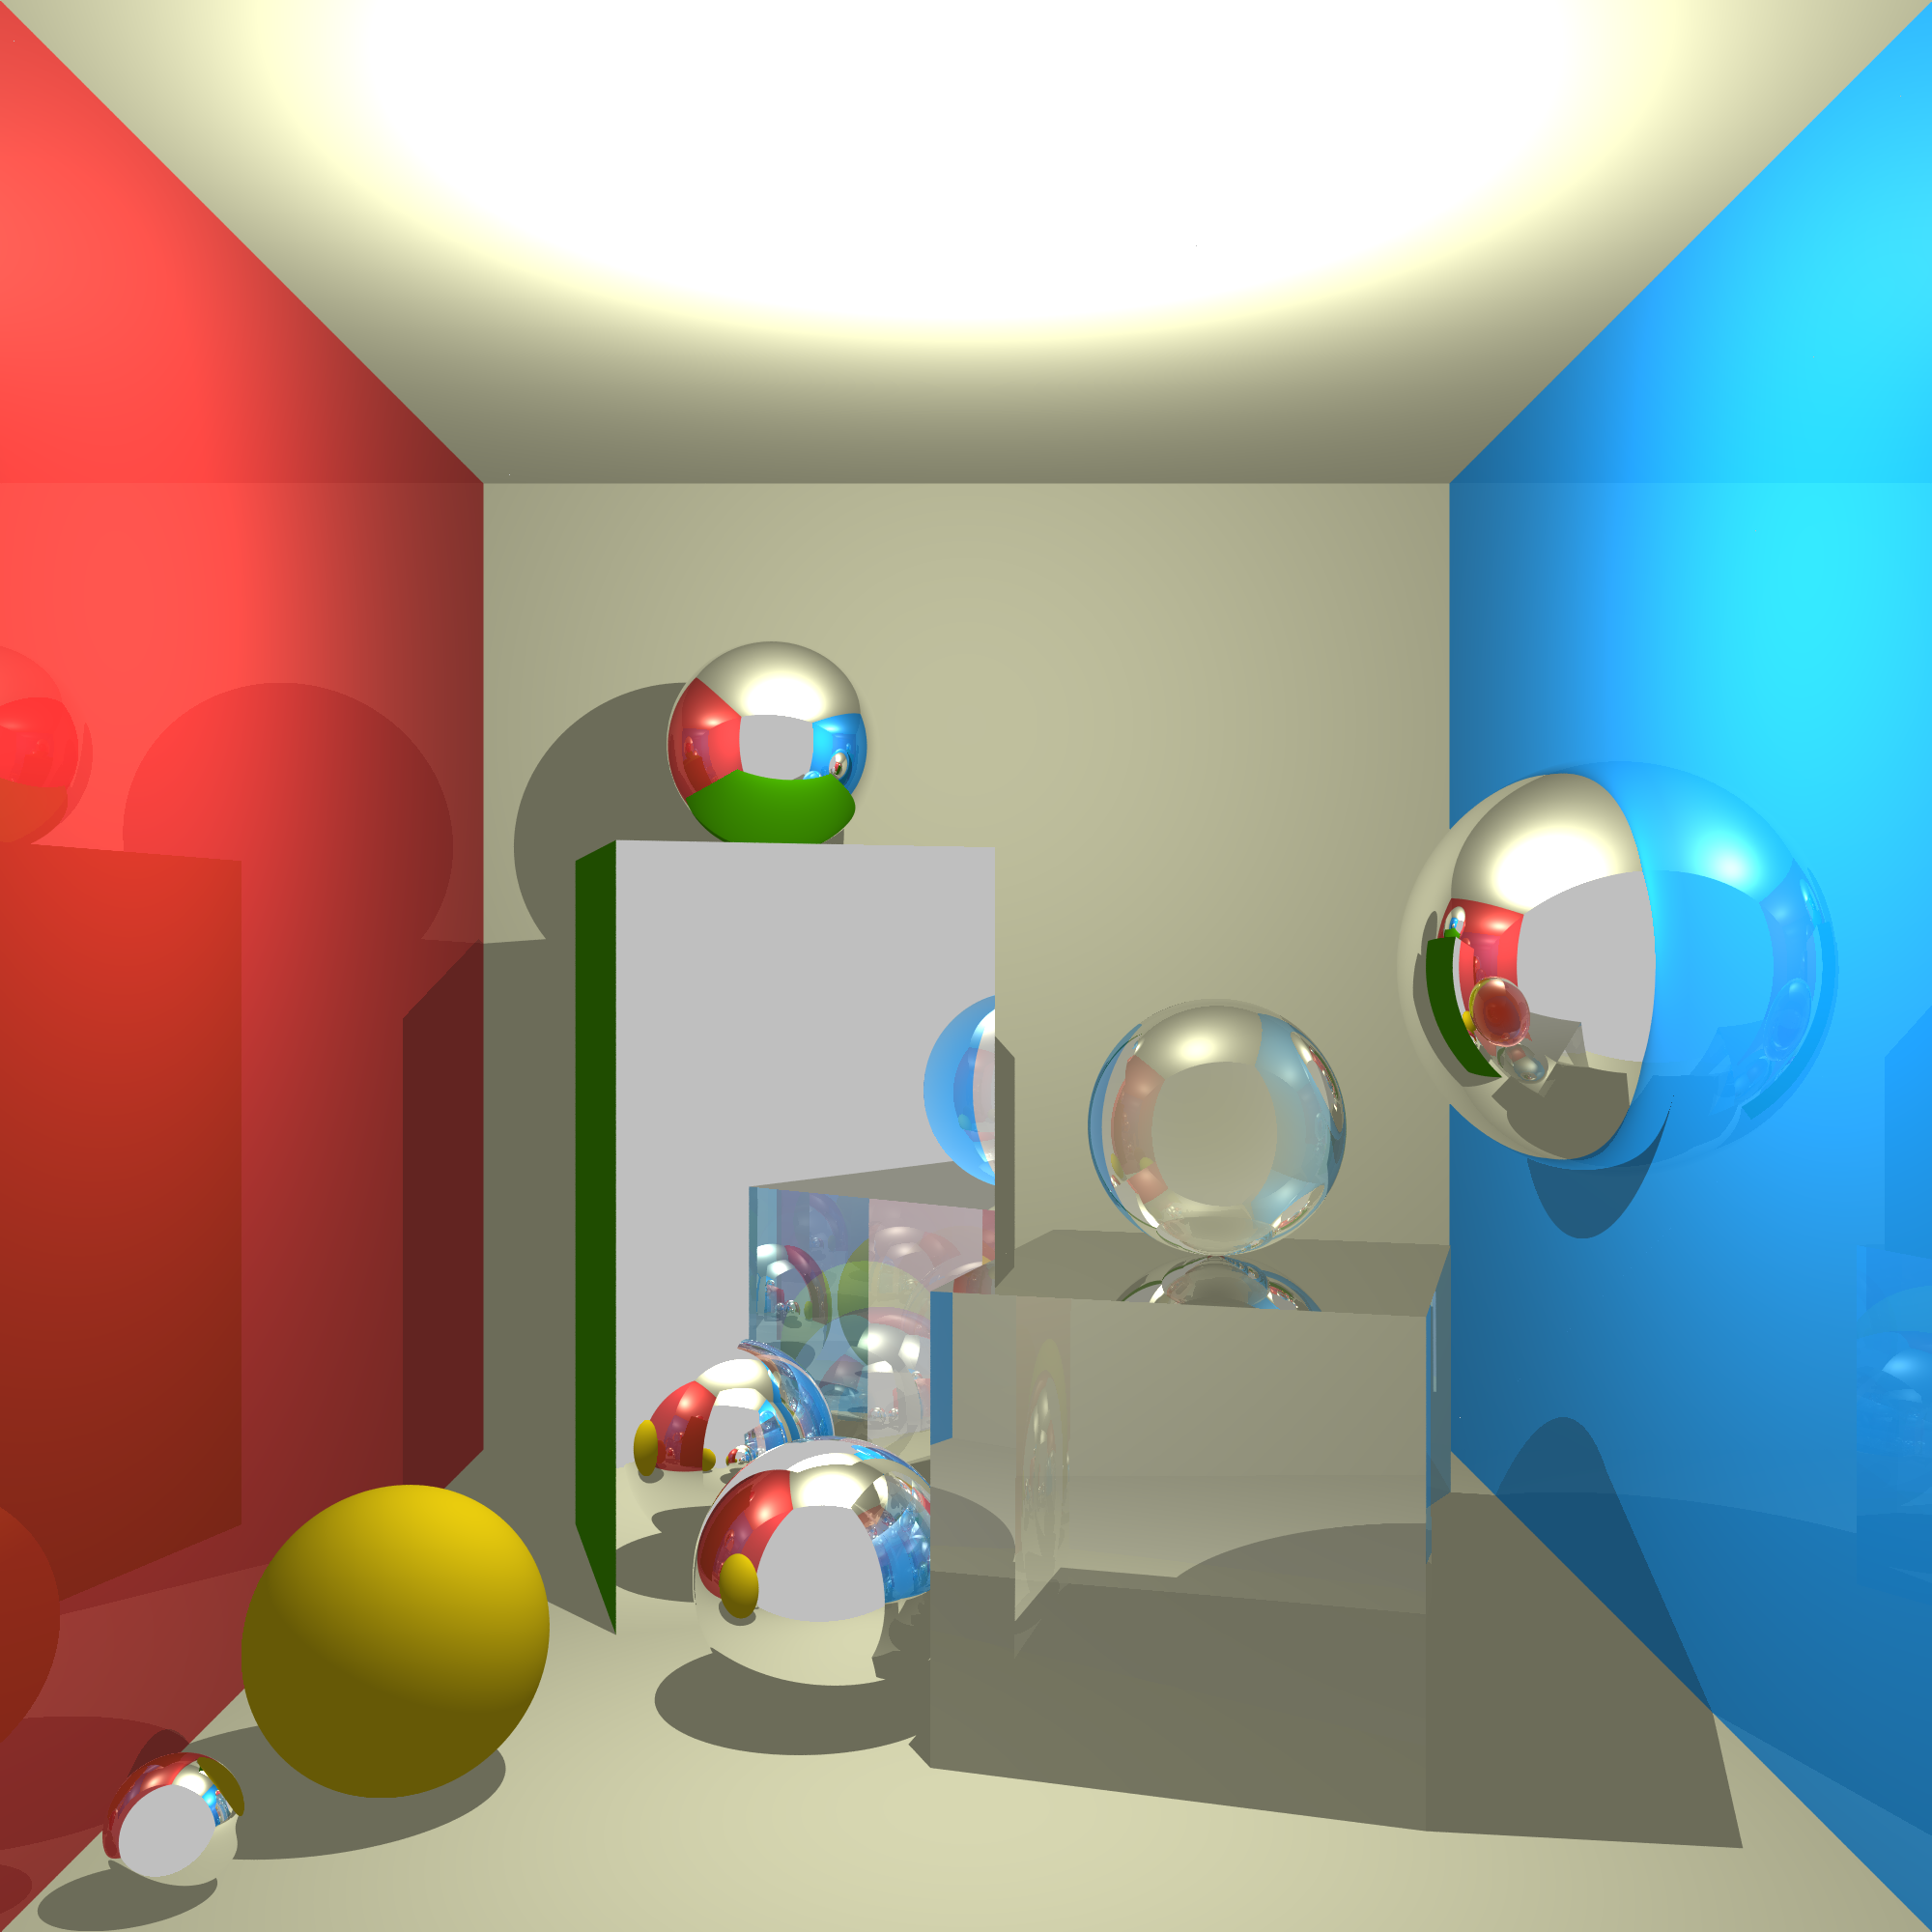
\includegraphics[width=0.4\linewidth]{img/glass_awesome.png}
\caption{Glass: refraction and reflection}
\end{figure}


\section{Soft shadows}
\subsection{Uniform light sources}
The following scenes were processed for a 500x500 resolution without anti-aliasing.
\begin{figure}[H]
\minipage{0.33\textwidth}
    \centering
    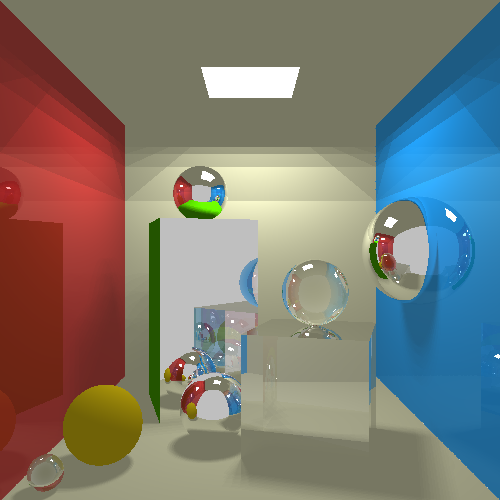
\includegraphics[width=\linewidth]{img/shadows/16.png}
    \caption{16 lights, uniform (8700 ms)}
\endminipage\hfill
\minipage{0.33\textwidth}
    \centering
    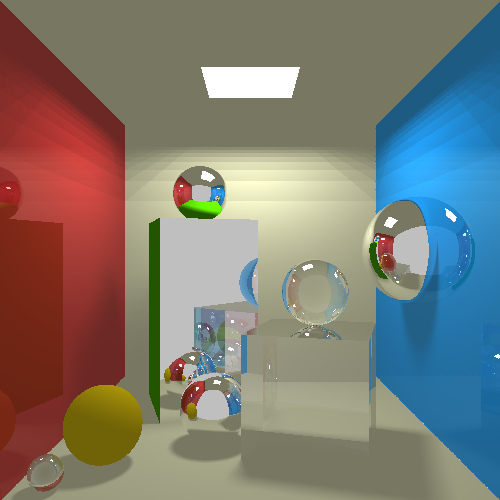
\includegraphics[width=\linewidth]{img/shadows/64.png}
    \caption{64 lights, uniform (30 600 ms)}
\endminipage\hfill
\minipage{0.33\textwidth}
    \centering
    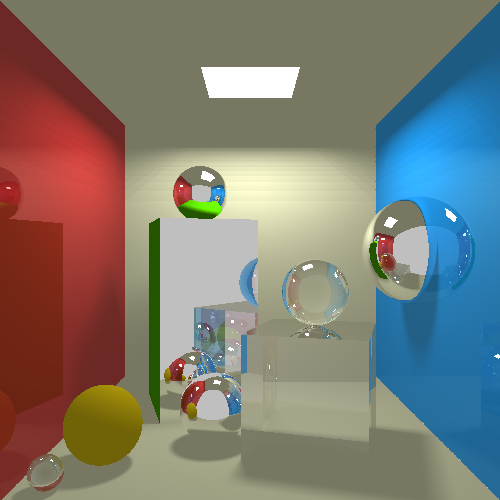
\includegraphics[width=\linewidth]{img/shadows/256.png}
    \caption{256 lights, uniform (118 500 ms)}
\endminipage\hfill
\end{figure}

\subsection{Jittered light sources}
\begin{figure}[H]
\minipage{0.33\textwidth}
    \centering
    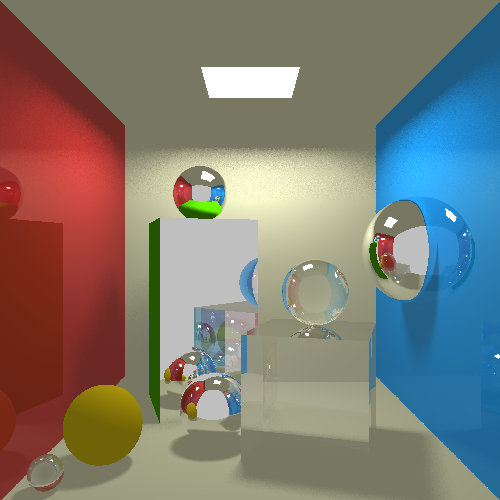
\includegraphics[width=\linewidth]{img/shadows/16_jittered.png}
    \caption{16 lights, jittered (9400 ms)}
\endminipage\hfill
\minipage{0.33\textwidth}
    \centering
    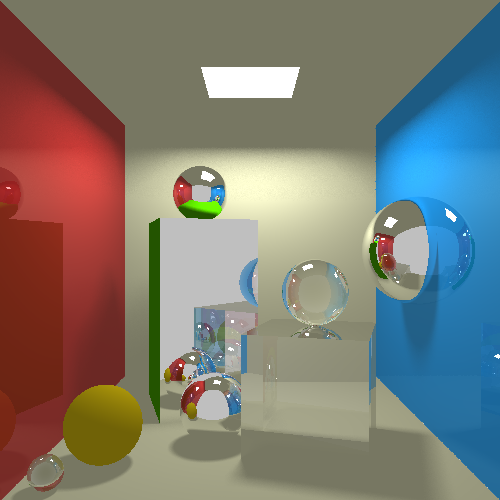
\includegraphics[width=\linewidth]{img/shadows/64_jittered.png}
    \caption{64 lights, jittered (33 600 ms)}
\endminipage\hfill
\minipage{0.33\textwidth}
    \centering
    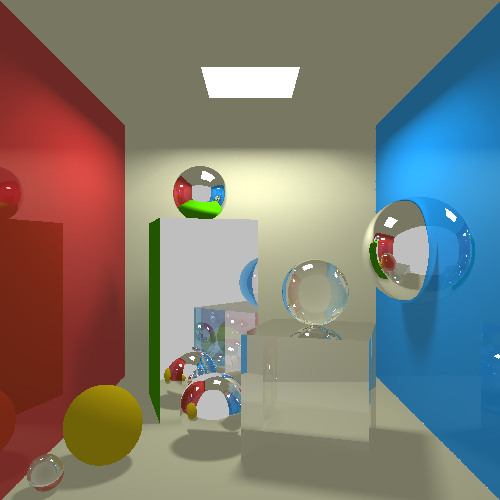
\includegraphics[width=\linewidth]{img/shadows/256_jittered.png}
    \caption{256 lights, jittered (128 600 ms)}
\endminipage\hfill
\end{figure}

%\begin{figure}[H]
%\centering
%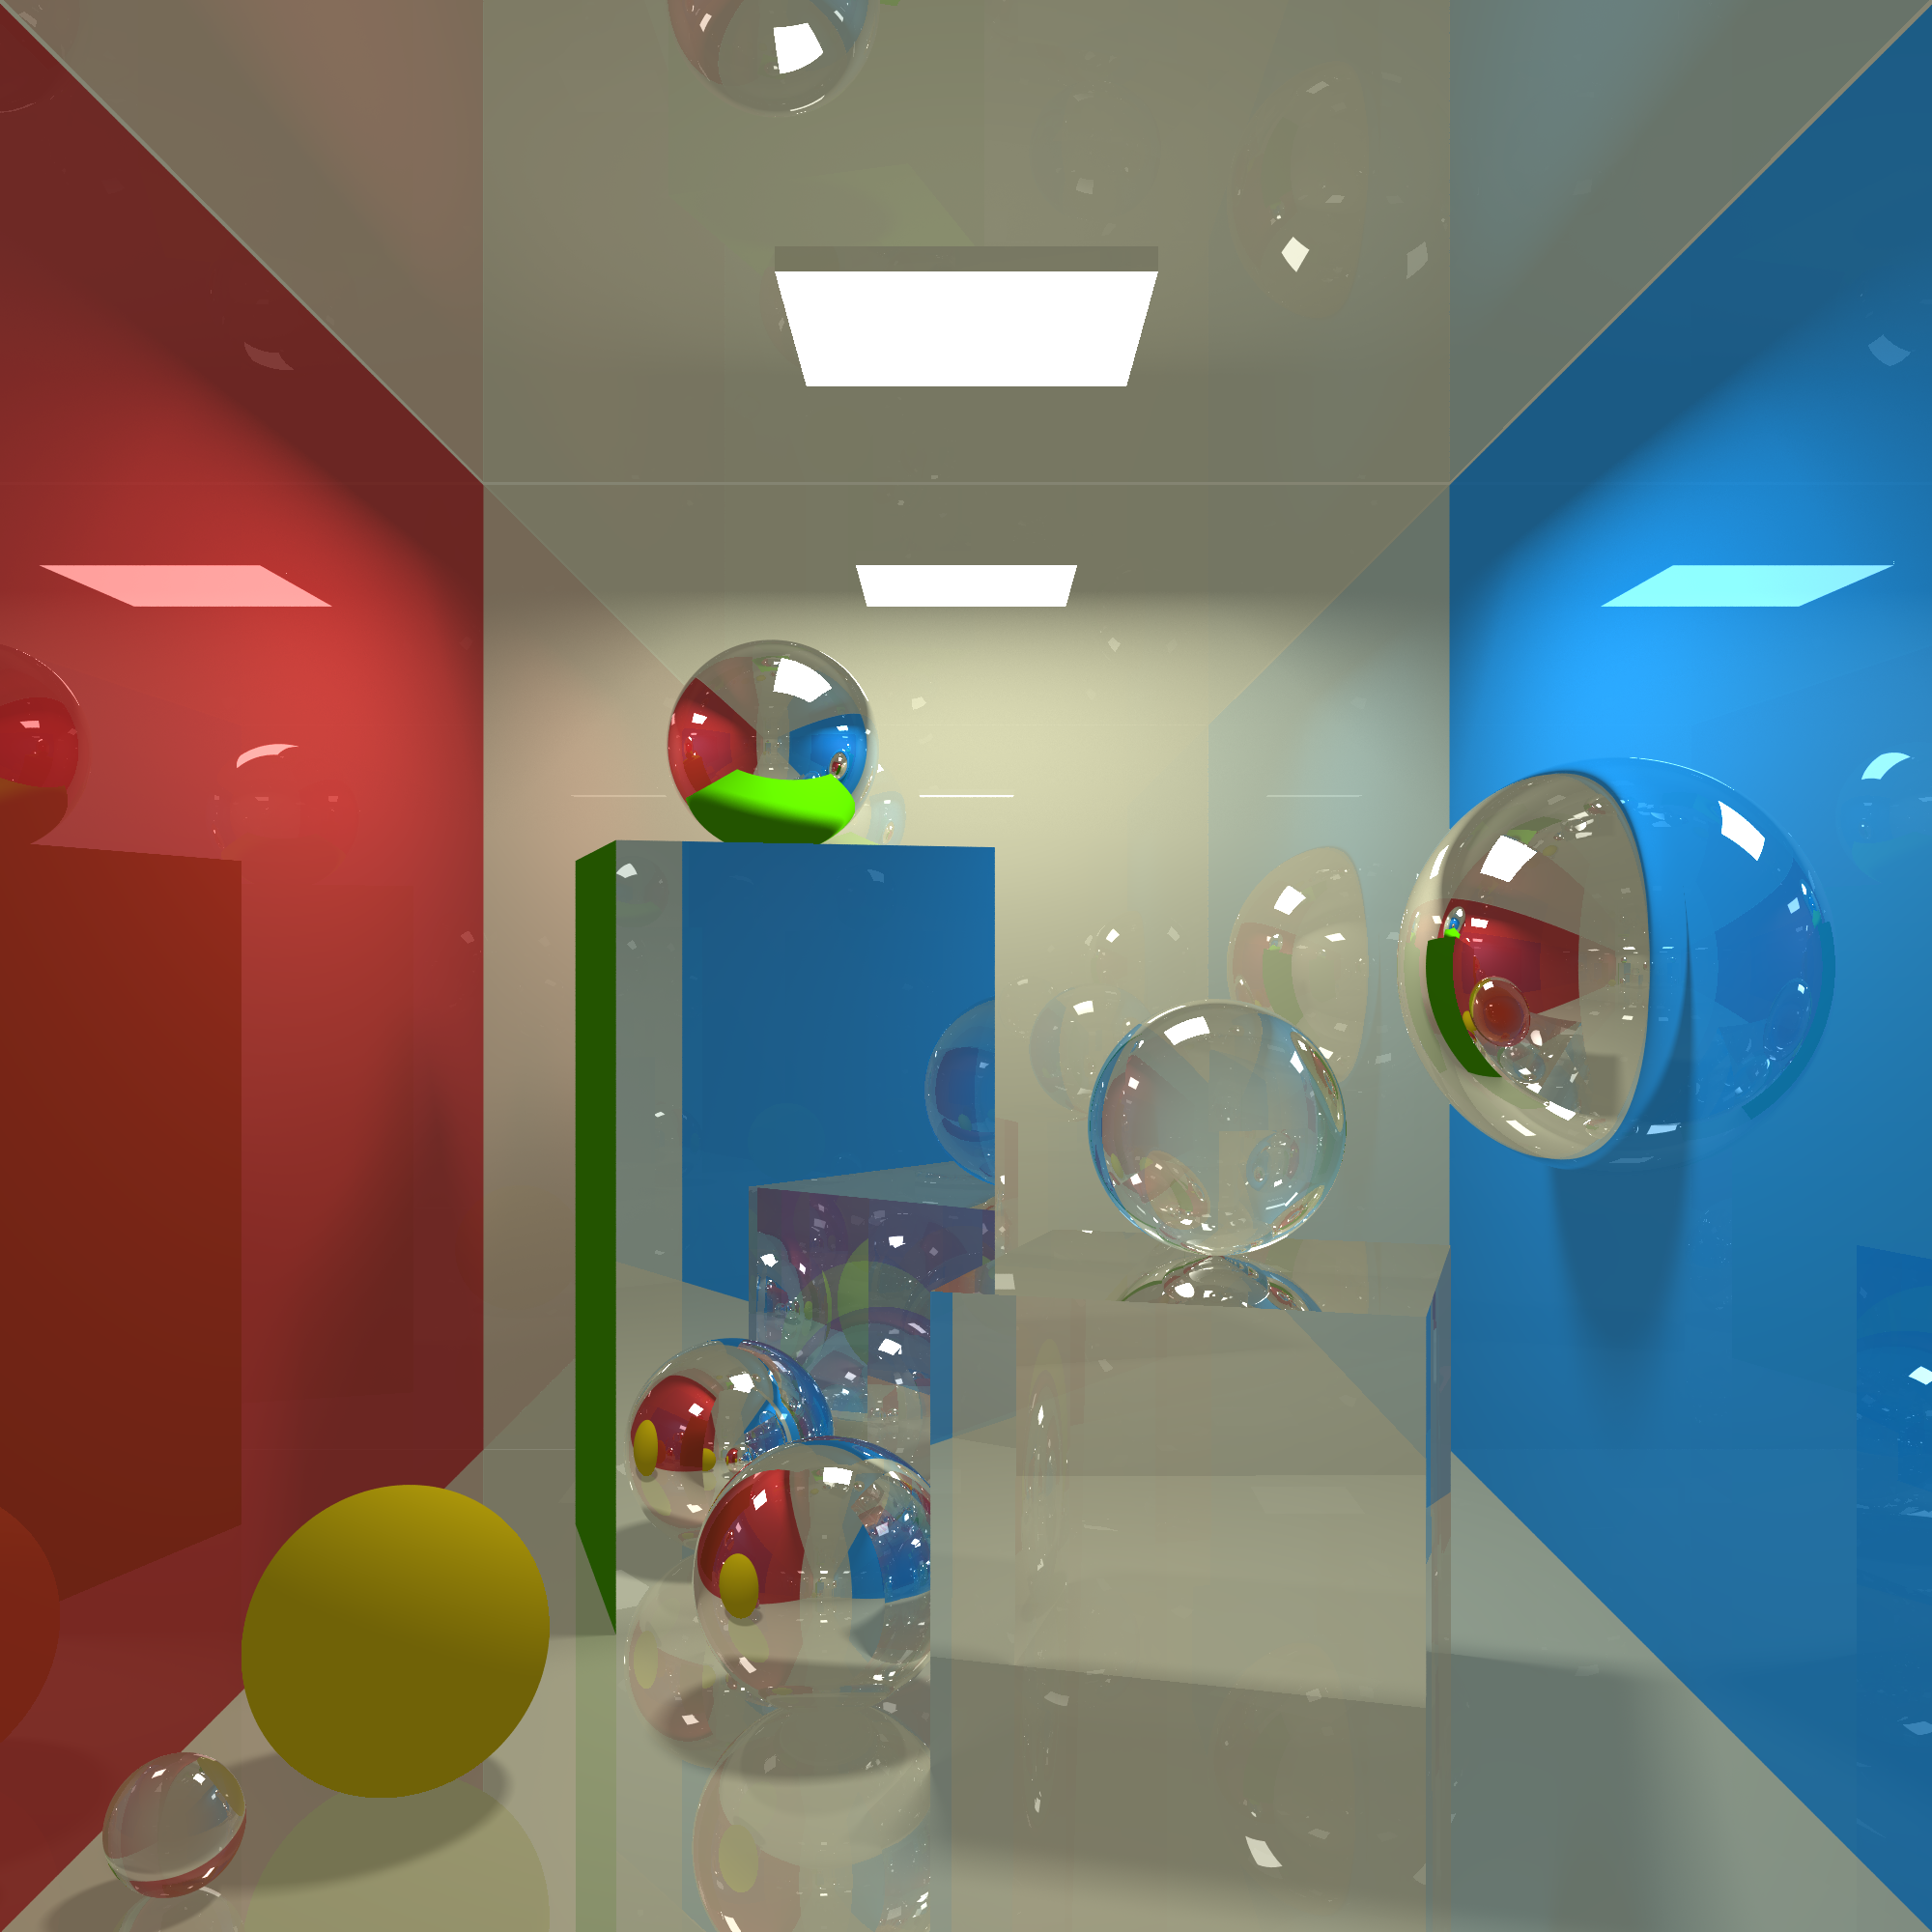
\includegraphics[width=0.4\linewidth]{img/final.png}
%\caption{Final scene}
%\end{figure}


    %\backmatter
\end{document}
